
\chapter{The geometry of coherent risk measures}
\label{chapter_finite_dimensional}

In this chapter, we first carefully set up the probability notation for the rest of the thesis. The impatient reader can skip over the section and refer to it only upon encountering difficulties in comprehension.

Then, we describe a geometric way to represent risk measures on random variables. This geometric viewpoint is then used to prove the Kusuoka representation for finite dimensional probability spaces with uniform probability distributions.

\section{Basic probability definitions and notations}
This section sets down and discusses basic probability definitions and notations.

\subsection{Probability space}
We set up the notations for Kolmogorov's probability axiomatization. For a detailed introduction to probability along this axiomatization, the reader is referred to \cite{chungCourseProbabilityTheory2001a}.

\begin{notn}\label{notn:probspace}
\((S, \mathcal{B}, \nu)\) is a \textbf{probability space}, with nonempty \(S\) as \textbf{state space}, \(\mathcal{B}\) a \textbf{\(\sigma\)-algebra} on \(S\), and \(\nu\) a \textbf{probability measure} on \((S, \mathcal{B})\). The \textbf{events} of $S$ are the elements of $\mathcal{B}$.
\end{notn}

\begin{conv}
If \(S\) is countable, then unless otherwise noted, we assume \(\mathcal{B} = 2^S\), that is, all subsets of \(S\) are measurable, and \(\forall \omega\in S, \nu(\{\omega\} ) > 0\), that is, all states have nonzero probability. This is an assumption of \textbf{nondegeneracy}.
\end{conv}

\begin{defn}
Any \(B \in \mathcal{B}\) with \( \nu(B) > 0\) is \textbf{non-atomic} if and only if \(\exists C \in \mathcal{B}\), such that \(C \subseteq B, \nu(B) > \nu(C) > 0\). In other words, it has a subevent with smaller, but still nonzero, probability. \(S\) is \textbf{atomless} if and only if all of its subsets with nonzero probability are non-atomic.
\end{defn}

\begin{remark}
	In particular, if $S$ is countable, then it is not atomless. In fact, it is the opposite of atomless, as every \(B \in \mathcal{B}\) with \( \nu(B) > 0\), any singleton subset of $B$ is atomic.
\end{remark}

\begin{conv}
Random variables, unless otherwise noted, are real, that is, they are real measurable functions on \(S\). In order to precisely define real measurability, we must specify a $\sigma$-algebra on $\mathbb{R}$, which we choose to be the set of Borel measurable sets of $\mathbb{R}$. In general, whenever necessary to formalize $\mathbb{R}^n$-measurability, we choose the set of Borel measurable sets of $\mathbb{R}^n$.
\end{conv}

\begin{conv}
Unless otherwise noted, $(X_n)$ denotes a sequence of independent and identically-distributed real random variables, indexed by $n$, that has the same distribution as $X$. The index $n$ ranges over $\mathbb{N}$.
\end{conv}

\begin{defn}
$(X_n)$ is the \textbf{IID process} of $X$. In general, any sequence of random variables is a \textbf{stochastic process}.
\end{defn}

\begin{notn}
The constant-one random variable is \(\mathds{1}\), such that \(\forall \omega\in S, \mathds{1}(\omega) = 1\). We abuse notation slightly, so that if there is no confusion, any constant $c$ can also denote the corresponding constant random variable $c\cdot \mathds{1}$.
\end{notn}

\subsection{Probability distributions}
\label{sec:prob_dist}
In probability theory, the underlying probability space is often immaterial for the problem that is being studied. As Terence Tao noted \cite{tao254ARandomMatrices2010}, probability theory can be said to be the study of measure spaces with measure one, but that is like saying number theory is the study of finite strings.

In particular, consider a coin, and let $X$ represent the number of heads that come up if it is flipped once. Then, if the coin is fair, we have $Pr(X = 0) = Pr(X=1) = \frac 1 2$. This can be formalized by defining an underlying probability space $S = \{1, 2\}$, with $\nu(1) = \nu(2) = \frac 1 2$, and $X(i) = i-1$. However, all this formality accomplishes little in the way of understanding the probabilistic behavior of $X$.

The part of $X$ that is of concern in probability theory is its distribution, that is, the probability of events involving $X$. For this particular $X$, its distribution is completely determined by $Pr(X = 0) = Pr(X=1) = \frac 1 2$.

In general, a real random variable is well-described by its probability measure:
\begin{defn}
Given a real random variable $X$, its associated \textbf{probability measure} $\mu_X$ is defined by 
\begin{equation}
\mu_X(E) = Pr(X \in E)
\label{eq:probability_measure}
\end{equation}
for any Borel measurable $E\subseteq \mathbb{R}$.
\end{defn}

It is a standard result in measure theory that $\mu_X$ is determined by the cumulative distribution function $F_X$:
\begin{defn}\label{defn:CDF}
Given a real random variable $X$, its \textbf{cumulative distribution function} (CDF) is defined by 
\begin{equation}
F_X(x) = Pr(X\le x) = Pr(X \in (-\infty, x]) = \nu(X^{-1}((-\infty, x]))
\label{eq:CDF}
\end{equation}
\end{defn}

It is a standard result in probability that the set of all possible CDF is the set of monotonically increasing, right-continuous real functions $F:\mathbb{R}\to[0, 1]$, such that $\lim_{x\to -\infty}F(x) = 0, \lim_{x\to +\infty}F(x) = 1$.

Due to possible jump discontinuities, the inverse of $F_X$ is not uniquely defined. The standard disambiguation is by demanding $F_X^{-1}$ to be left-continuous:
\begin{defn}
	Given a real random variable $X$, its \textbf{quantile function} $F_X^{-1}:[0, 1] \to [-\infty, \infty]$ is defined by 
	\begin{equation}
	F_X^{-1}(q) = \inf \{t : F_X(t) \ge q\} 
	\label{eq:quantile}
	\end{equation}
	Note that $	F_X^{-1}(0) = -\infty$, and $F_X^{-1}(1) = \esssup(X)$, which could be $+\infty$. For all $0<\alpha < 1$ cases, $F_X^{-1}(\alpha)$ is real-valued.
\end{defn}

\begin{ex}\label{ex:var}
For any $0\le\alpha\le 1$, the \textbf{value-at-risk at level $\alpha$} of a random variable $X$ is $\var_\alpha(X) = F_X^{-1}(\alpha)$.
\end{ex}


\begin{defn}
Given $X$, let $(X_n)$ be its IID process, then for any $n\in \mathbb{N}$, the $n$-th \textbf{empirical cumulative distribution function} of $X$ is a random CDF defined by
\begin{equation}
F_{n}(x)={\frac {1}{n}}\sum _{i=1}^{n}1_{(-\infty ,x]}(X_{i})
\label{eq:empirical_CDF}
\end{equation}
where for any set $C$, $1_C$ is its indicator function. 
\end{defn}

\begin{defn}
\label{defn:empirical_process}
The $n$-th \textbf{empirical measure} of $X$ is the discrete measure
\begin{equation}
\mu_{X, n} = {\frac {1}{n}}\sum _{i=1}^{n}\delta_{X_i}
\label{eq:empirical_measure}
\end{equation}
where $(X_n)$ is the IID process of X, and for any element $x$, $\delta_x$ is the Dirac delta measure, defined by 
\begin{equation*}
\forall E\subseteq \mathcal{B}, 
\quad
\delta_x(E) = \begin{cases}
1 \quad \text{if } x\in E,\\
0 \quad \text{else.}
\end{cases}
\end{equation*}

For each $\mu_{X, n}$, let $L_n$ be a discrete random variable that has probability measure equaling $\mu_{X, n}$, then the sequence of $(L_n)$ defines the \textbf{empirical process} of $X$.
\end{defn}

\begin{remark}
Since the empirical CDF $F_{X, n}$, and the empirical measure $\mu_{X, n}$, of $X$, are based on the IID process of $X$, which is itself random, $F_{X, n}$ and $\mu_{X, n}$ are thus random functions, while $F_X$ and $\mu_X$ are deterministic.
\end{remark}

\begin{conv}
Some functionals $\mathcal{F}$ on real random variables $X$, such as the expectation, are defined purely by the probability measure $\mu_X$ of $X$, which is determined by $F_X$. As such, we can unambiguously abuse notation:
\begin{equation}
\mathcal{F}(X) = \mathcal{F}(F_X) = \mathcal{F}(\mu_X) 
\end{equation}
As will be defined in Definition \ref{defn:risk_functional_properties}, this is equivalent to saying $\mathcal{F}$ is \textbf{law invariant}.

As an example, for any real random variable $X\in\mathscr{L}^1$, with CDF $F_X$ and corresponding probability measure $\mu_X$ on $\mathbb{R}$, we have three equivalent definitions of expectation:
\begin{equation}
	\label{eq:expectation_integral}
	\begin{aligned}
	  \mathbb{E}(X) &= \int_S X(\omega) d\nu(\omega) \\
	= \mathbb{E}(F_X) &= \int_{[0, 1]} F_X^{-1}(\alpha)d\alpha \\
	= \mathbb{E}(\mu_X) &= \int_\mathbb{R} x d\mu_X(x) 
	\end{aligned}
\end{equation}
\end{conv}

\begin{ex}
\label{ex:IID_average}
The \textbf{$n$-th empirical mean} of $X$ is 
$$\frac 1 n \sum_{i = 1}^n X_i = \mathbb{E}(F_{X, n}).$$

To say $X$ satisfies the Strong Law of Large Numbers (SLLN) is to say that 
$$\mathbb{E}(F_{X, n})\asconv \E(F_X)=\E(X),$$
where $\asconv$ denotes almost-sure convergence.
\end{ex}

This is the first example of the general phenomenon, where, if $X$ is a "well-behaved" random variable, $F_{X, n}$ converges in some sense to $F_X$ as $n\to \infty$. That is, the empirical distribution $F_{X, n}$ approximates certain aspects of the true distribution $F_X$ with arbitrary precision, as $n\to \infty$.

In Chapter \ref{chapter_clt}, we will prove several generalizations of the Central Limit Theorem that exhibit this general phenomenon.

\subsection{Hilbert space of real random variables}
\begin{notn}
Given a probability space \((S, \mathcal{B}, \nu)\), let $\LL(S)$ be the space of all real random variables over $S$. Let \(\mathscr{L}^p(S)\) be the space of all real random variables with finite $p$-moment. When no confusion could arise, $S$ is omitted.
\end{notn}

The case of $p=2$ is special, as \(\mathscr{L}^2\) is a Hilbert space of square-integrable real functions of $S$.
\begin{conv}
	Unless otherwise noted, real random variables have finite variance. That is, we restrict our attention to elements of $\mathscr{L}^2(S)$
\end{conv}

\begin{notn}
	The inner product on \(\mathscr{L}^2\) is \(\left<X, Y \right> = \mathbb{E}(XY)\).
\end{notn}

\begin{notn}\label{notn:subsets_of_l2}
Certain special sets are:
\begin{itemize}
	\item \(\mathscr{E}_{=c} = \{X \in \mathscr{L}^2 : \mathbb{E}(X) = c\} \).
	\item \(\mathscr{L}^2_+ = \{X \in \mathscr{L}^2 : X \ge 0\} \). This is called the nonnegative quadrant of \(\mathscr{L}^2\).
	\item \(\mathscr{D} = \mathscr{E}_{=1} \cap \mathscr{L}^2_+\). This is the set of all random variables that are nonnegative, and have expectation one. If \(S\) is finite, then it is a simplex, which is often written with the letter \(\Delta\) ("Delta", the Greek letter that looks like a simplex).
	\item For any $p \in [1, \infty)$, \(\mathscr{U}_p = \{X\in \mathscr{L}^2 : \E(|X|^p) \le 1\} \). This is the unit ball in \(p\)-norm. By H\"older's inequality, for all $p \ge q \ge 1$, $\mathscr{U}_p\subseteq \mathscr{U}_q$.
	\item \(\mathscr{U}_\infty = \{X \in \mathscr{L}^2(S ) : -1 \le X \le 1\text{ almost surely}\} \). It can be thought of as the limit that is, $$\mathscr{U}_\infty = \lim_{p\to\infty} \mathscr{U}_p = \bigcap_{p\ge 1}\mathscr{U}_p$$.
\end{itemize}
\end{notn}

\subsection{Functionals on random variables}
\begin{defn}\label{defn:risk_functional_properties}
We define special properties of functional \(\mathcal{F}\) on \(\mathscr{L}^2\). In the following list, these conditions are added to the front: $\forall c\in \mathbb{R}, Z, Z'\in \mathscr{L}^2$.
\begin{enumerate}[(1)]
	\item \textbf{Subadditivity.} $\mathcal{F}\left(Z + Z'\right) \leq \mathcal{F}(Z)+ \mathcal{F}\left(Z^{\prime}\right)$.
	\item \textbf{Positive homogeneity.} $\mathcal{F}(\lambda Z)=\lambda \mathcal{F}(Z)$, for all $\lambda \ge 0$. Note that this implies $\mathcal{F}(0) = 0$
	\item \textbf{Convexity.} $\mathcal{F}\left((1-\lambda) Z+\lambda Z^{\prime}\right) \leq(1-\lambda) \mathcal{F}(Z)+\lambda \mathcal{F}\left(Z^{\prime}\right)$, for all $0\le \lambda \le 1$.
	\item \textbf{Sublinearity.} Subadditive and positive homogeneous. This implies convexity.
	\item \textbf{Monotonicity.} $\mathcal{F}(Z) \leq \mathcal{F}\left(Z^{\prime}\right)$ whenever $Z \leq Z^{\prime}$ $\nu$-a.s..\newline That is, when $\nu(\{s \in S | Z(s) \leq Z^{\prime}(s)\})=1$
	\item \textbf{Translation invariance.} $\mathcal{F}(Z+c)=\mathcal{F}(Z)+c$.
	\item \textbf{Coherence.} Sublinear, monotone, and translation invariant.
	\item \textbf{Closedness.} $\left\{Z \in \mathscr{L}^{2} | \mathcal{F}(Z) \leq c\right\}$ is closed. Note that the topology on $\mathscr{L}^{2}$ is defined by its inner product.
	\item \textbf{Risk aversity.} \(\mathcal{F}\ge \mathbb{E}\).
	\item \textbf{Strict risk aversity.} \(\mathcal{F}\ge \mathbb{E}\), with equality reached \textit{only} for almost surely constant random variables.
	\item \textbf{Law invariance.} $X\disteq Y$ implies $\mathcal{F}(X) = \mathcal{F}(Y)$.
\end{enumerate}
\end{defn}

Each of these properties can be interpreted as formalizing practical properties of risk measures:
\begin{enumerate}[(1)]
	\item \textbf{Subadditivity}: "merger does not create extra risk". See \cite{artznerCoherentMeasuresRisk1999} for a detailed discussion.
	\item \textbf{Positive homogeneity}: doubling the outcome in all cases doubles the risk. This is sometimes called "scale invariance".
	\item \textbf{Convexity}: iversification can only decrease risk, that is, holding stocks in a certain proportion has less risk compared to holding them separately in the same proportion.
	\item \textbf{Sublinearity}: Positively homogeneous and convex.
	\item \textbf{Monotonicity}: if in all cases, the outcome is not better, then the risk is not lower.
	\item \textbf{Translation invariance}: adding a sure loss of $c$ increases risk by $c$.
	\item \textbf{Coherence}: to be interpreted in Section \ref{sec:crm}.
	\item \textbf{Closedness}: A technical assumption. A closed risk measure has convenient analytical properties, such as being lower semicontinous, and satisfying a Fatou's lemma. See \cite[Theorem 2]{kusuokaLawInvariantCoherent2001} for details.
	\item \textbf{Risk aversity}: As noted in Section \ref{sec:other_traditions}, in classical decision theory, a rational agent maximizes its expectation of utility, and is unconcerned with variances, no matter how extreme. Humans, in contrast, are often "risk averse", that is, they often give up a higher expectation if the variance is too great, indicating that they think such situations have a higher risk than the mere expectation.
	\item \textbf{Strict risk aversity}: a more exacting risk aversity. If $X$ has any non-determinancy in its outcome, it is regarded as more risky than a sure loss of $\mathbb{E}(X)$.
	\item \textbf{Law invariance}: As noted in Section \ref{sec:prob_dist}, the distribution functions of random variables are all that matters in probability, and so any risk measure meaningful in probability must be insensitive to any change of random variable that leaves its distribution unchanged, that is, it must be law invariant.
	
For more extensive interpretations of these properties, the reader is directed to the references in \cite{gianinRiskMeasuresGexpectations2006}.

\end{enumerate}


\section{Coherent risk measures (CRM)}
\label{sec:crm}

\subsection{Importance of coherence}
The idea of coherence in risk measurement was first proposed in the context of financial mathematics by \cite{artznerCoherentMeasuresRisk1999}. Artzner explicitly argued against using \var, due to its incoherence.

\begin{ex}[$\var$ is incoherent]
Let $Pr(X=-1) = Pr(X=+1) = 0.5$, and $Y$ be an independent copy of $X$, then 
$$\var_{0.49}(X+Y) = 0 > \var_{0.49}(X) + \var_{0.49}(Y) = -2.$$
\end{ex}

Requiring a risk measure to be coherent incorporates several intuitions in judging the risk of financial products, and by extension, risky non-financial situations. Detailed interpretation of these risk measurement intuitions are found in \cite{artznerCoherentMeasuresRisk1999}. 

\subsection{Conditional VaR (CVaR)}
The conditional value-at-risk (CVaR) was proposed to be a coherent alternative to \var, and has achieved a preeminent position in financial risk management. Intuitively, the CVaR at level $\alpha$ of a random loss $X$ is the expectation of loss, conditional on the loss being the worst $(1-\alpha)$ cases. That is, 
\begin{equation}
\label{eq:preliminary_cvar}
\cvar_\alpha(X) = \mathbb{E}(X | X > F_X(\alpha))
\end{equation}
for any $0\le\alpha < 1$. Note that when $\alpha = 0$, $F_X(\alpha)= -\infty$, and so $\mathbb{E}(X | X > F_X(\alpha)) = \mathbb{E}(X)$.

\begin{remark}
We will concentrate on the cases of $0<\alpha < 1$ when discussing $\cvar_\alpha$, since $\alpha = 0$ gives expectation, and $\alpha = 1$ gives essential supremum, both cases being often easier to handle.
\end{remark}

This naive definition unfortunately does not work when $X$ is atomic, because in such cases, $F_X$ has jump discontinuities where the value of $F_X(\alpha)$ is ambiguous. Fortunately, there is a more general definition that overcomes such problems \cite[Definition 3]{rockafellarConditionalValueatriskGeneral2002}:

\begin{defn}\label{defn:cvar}
For any $0\le\alpha < 1$.
\begin{equation}
\label{eq:def_cvar}
\cvar_\alpha(X) = \mathbb{E}(X^{(\alpha)})
\end{equation}
where $X^{(\alpha)}$ is a random variable with the CDF 
\begin{equation}
\label{eq:def_cvar_CDF}
F_{X^{(\alpha)}}(x) =  \left( \frac{F_X(x)-\alpha}{1-\alpha}\right)^+
\end{equation}
\end{defn}

Intuitively, to get the graph of $F_{X^{(\alpha)}}$, take the graph of $F_X$, truncate it above the $y=\alpha$ line, and stretch it down to fill the $0 \le y \le 1$ stripe again.

\begin{theorem}[$\cvar$ is coherent, strictly risk averse, and law invariant]
For any $0 \le\alpha\le 1$, $\cvar_\alpha$ is coherent, strictly risk-averse, and law invariant.
\end{theorem}

The only difficulty is in proving the subadditivity of $\cvar$. To show it, we utilize equivalent ways to define $\cvar$, offering different perspectives on it. The most useful ones for our purpose are

\begin{prop}[Equivalent formulations of $\cvar$]
For any real random variable $X$, and any $0\le \alpha<1$, we have 
	\begin{equation}\label{eq:cvar_defs}
		\cvar_\alpha(X) = 
		\min_{s \in\mathbb{R}}
			\left(s+\frac{1}{{\overbar{\alpha}}} \mathbb{E}\left((X-s)^{+}\right)\right) = 
		\frac{1}{{\overbar{\alpha}}} \int_\alpha^1 F_X^{-1}(q) dq
	\end{equation}
\end{prop}
\begin{proof}
See \cite[Theorem 10]{rockafellarConditionalValueatriskGeneral2002} and \cite[Proposition 3.2]{acerbiCoherenceExpectedShortfall2002}. 
\end{proof}

As an example of the power of such representation, the subadditivity of $\cvar$ is now immediate:

\begin{proof}
	For any $\alpha \in (0, 1)$, and real random variables $X, Y$, let 
	$$s_1 \in \argmin_{s\in\mathbb{R}} \left(s+\frac{1}{{\overbar{\alpha}}} \mathbb{E}\left((X-s)^{+}\right)\right),
	s_2 \in \argmin_{s\in\mathbb{R}} \left(s+\frac{1}{{\overbar{\alpha}}} \mathbb{E}\left((Y-s)^{+}\right)\right),$$
	and 
	$$s_0 = s_1 + s_2,$$  
	then we use the minimization definition of CVaR (Equation \ref{eq:cvar_defs}):
	\begin{align*}
	\cvar_\alpha( X+ Y) &= 
		\min_{ s \in\mathbb{R}}
		\left( s+\frac{1}{{\overbar{\alpha}}} \mathbb{E}\left((X + Y-s)^{+}\right)\right)\\
		&\le s_0 + \frac{1}{{\overbar{\alpha}}} \mathbb{E}\left((X + Y-s_0)^{+}\right)\\
		&= s_1+s_2 + \frac{1}{{\overbar{\alpha}}} \mathbb{E}\left((X - s_1 + Y-s_2)^{+}\right)\\
	  &\le  \left(s_1+\frac{1}{{\overbar{\alpha}}} \mathbb{E}\left((X-s_1)^{+}\right)\right)
	  +  \left(s_2+\frac{1}{{\overbar{\alpha}}} \mathbb{E}\left((Y-s_2)^{+}\right)\right)\\
	  &=  \cvar_\alpha( X) +  \cvar_\alpha(Y),
	\end{align*}
	where we used the fact that for any two real numbers $x,y$, $(x+y)^+ \le x^+ + y^+$.
\end{proof}

\begin{prop}[Continuity of CVaR]
For any real random variable $X$, $\cvar_\alpha(X)$ is a continuous function on $0 \le \alpha\le 1$.
\end{prop}
\begin{proof}
By the integral definition of CVaR, $\cvar_\alpha(X)$ is continuous on $0 \le \alpha < 1$.

If $\esssup(X) < \infty$, then for any $\epsilon> 0$, there exists $\alpha_0$ such that any $\alpha > \alpha_0$, $F_X^{-1}(\alpha) >\esssup(X) -\epsilon $, and so $\cvar_{\alpha}(X) > \esssup(X) -\epsilon$.

If $\esssup(X) = \infty$, the proof is similar, with an arbitrarily big $M$ replacing $\esssup(X) -\epsilon$.
\end{proof}

\subsection{The significance of CVaR}
There are representation theorems, often named "Kusuoka representation", with the following format: On any "nice" probability space $S$, any law invariant CRM $\mathcal{F}$ that is "nice" can be represented by  convex integrals of CVaR. 

Now we state this rigorously.

\begin{defn}\label{defn:kusuoka_rep}
Given a closed and sublinear functional \(\mathcal{F}\) on \(\mathscr{L}^2\), we say that it has a \textbf{Kusuoka representation} if and only if it can be represented as 
\begin{equation}
\mathcal{F}(X) = \sup_{\theta\in \Theta} \int_{[0, 1]} \text{\cvar}_\alpha(X) dm_\theta(\alpha) \quad \text{for all }X \in \mathscr{L}^2
\label{eq:kusuoka_rep}
\end{equation}
where \(\{m_\theta : \theta \in \Theta\} \) is a family of probability measures on \([0, 1]\).
\end{defn}

Kusuoka representation theorems in general state that, if \(S\) and \(\mathcal{F}\) satisfies certain conditions, then \(\mathcal{F}\) has a Kusuoka representation \cite[Section 2.2.4]{pflugModelingMeasuringManaging2008}. The original theorem has been generalized to dizzying heights of abstraction, which we will not review.

If the $\sup$ sign is removed, we obtain the class of spectral risk measures\footnote{Such representation is sometimes called Choquet representation, for example in \cite[Definition 2.48]{pflugModelingMeasuringManaging2008}.}, proposed in \cite{acerbiSpectralMeasuresRisk2002}:
\begin{defn}
A \textbf{spectral risk measure} is any $\mathcal{F}$ defined by a probability distribution $m$ on $[0, 1]$, and 
\begin{equation}
\mathcal{F} = \int_0^1 \cvar_\alpha dm(\alpha)
\end{equation}
\end{defn}

\begin{defn}
	Two random variables $X, Y: S\to \mathbb{R}$ are \textbf{comonotone} if for all $\omega, \omega'\in S$, 
	\begin{equation}
	(X(\omega) - X(\omega'))(Y(\omega) - Y(\omega')) \ge 0,
	\end{equation}
	that is, $X, Y$ rises and falls together.
	
	A risk measure $\mathcal{F}$ is comonotone additive if for any comonotone $X, Y$, 
	\begin{equation}
	\mathcal{F}(X + Y) = \mathcal{F}(X) + \mathcal{F}(Y).
	\end{equation}
\end{defn}

\begin{prop}[Kusuoka representation]
	\label{thm:kusuoka}
Any risk function with Kusuoka representation is a law invariant coherent risk measure. 

If the probability space $S$ is atomless, then the converse also holds.

A risk functional is a law invariant coherent and comonotone additive functional if and only if it is a spectral risk measure.
\end{prop}
\begin{proof}
See \cite[Theorem 3.1]{noyanKusuokaRepresentationsCoherent2015}.
\end{proof}

\section{The envelope representation of risk measures}
In math, there is a common duality between analysis and geometry. The risk measures, being analytical, have the dual representation as risk envelopes.

\begin{defn}
Given any nonempty subset \(\mathscr{F}\subseteq \mathscr{L}^2\), its associated \textbf{support function} is 
\[\sigma_{\mathscr{F}}(X) = \sup \{\left<X, F \right> | F \in \mathscr{F}\} \]
which we often write as \(\mathcal{F}\).

Given a functional \(\mathcal{F}\), if there exists some \(\mathscr{F}\subseteq \mathscr{L}^2\), such that \(\mathcal{F} = \sigma_{\mathscr{F}}\), then we say that it has an \textbf{envelope representation} \(\mathscr{F}\). 
\end{defn}

\subsection{The symmetry group on \(\mathscr{L}^2\)}
To describe the geometry of law-invariance, we define:
\begin{defn}
	The \textbf{symmetry group} on \(\mathscr{L}^2\) is 
	\begin{equation}
	\mathbb{G}=\{(\circ f) | f \text{ is a measure-preserving bijection on } S\}
	\label{eq:symmetry_group_on_L2}
	\end{equation}
\end{defn}

Then \(\mathbb{G}\) is a group that acts on \(\mathscr{L}^2\) on the right. This group action preserves distribution, that is,
\[\forall X \in \mathscr{L}^2, (\circ f)\in \mathbb{G}, X\circ f \text{ and } X \text{ have the same distribution}.\]
In particular, \(\mathbb{G}\)-action preserves:
\begin{itemize}
	\item law invariant functionals on \(\mathscr{L}^2\), such as the inner product and \(\mathbb{E}\);
	\item certain elements and subsets of \(\mathscr{L}^2\), such as \(\mathds{1}\), \(\mathscr{L}^2_+\), \(\mathscr{E}_{=1}\), and \(\mathscr{D}\).
\end{itemize}

If we think of \(\mathscr{L}^2\) as a linear subspace of \(\mathbb{R}^S\), then each element of \(\mathbb{G}\) acts on $\mathscr{L}^2$ by a permutation of the coordinates.

\subsection{Geometry of risk envelopes}
There is a bijection between certain risk measures and risk envelopes \cite[Section C.3]{hiriart-urrutyFundamentalsConvexAnalysis2001}:
\begin{align}
&\{\mathcal{F}\: | \: \mathcal{F}: \mathscr{L}^2\to (-\infty, \infty], \text{ sublinear and closed}\} \\
\leftrightarrow &
\{\mathscr{F} \:|\: \mathscr{F}\subseteq \mathscr{L}^2,\text{ nonempty, closed, and convex}\}
\end{align}
with the bijection given explicitly by 
\begin{equation}
\mathcal{F}(X ) = \sup_{Q \in \mathscr{F}} \left<X, Q \right> \quad \mathscr{F} = \{Q \in \mathscr{L}^2 : \left<X, Q \right>\le \mathcal{F}(X), \forall X \in \mathscr{L}^2 \}.
\end{equation}

\begin{remark}
	The sublinear and closed risk measures can be partially ordered by
\begin{equation}
\mathcal{F} \ge \mathcal{G} 
\quad \text{iff}\quad
\forall X \in \mathscr{L}^2, \mathcal{F}(X) \ge \mathcal{G}(X) 
\end{equation}
In terms of their risk envelopes, 
\begin{equation}
\mathcal{F} \ge \mathcal{G} 
\quad \text{iff}\quad
\mathscr{G} \subseteq \mathscr{F}
\end{equation}

With this ordering, the set of all sublinear and closed risk measures becomes a lattice \cite[Section 5.4]{williamsonFairnessRiskMeasures2019}. Its maximal element is the essential supremum, and its minimal element is the expectation. This explains the thesis title.
\end{remark}

The following proposition enumerates the correspondence between analytic properties of risk measure and geometric properties of its risk envelope. It is \cite[Proposition 7]{williamsonFairnessRiskMeasures2019}.

\begin{prop}
\label{prop:envelop_rep}
Suppose \( \mathcal{F} : \mathscr{L}^2 \to (-\infty , \infty ] \) is a sublinear, closed functional, with envelope representation 
\[\mathcal{F}(X ) = \sup_{Q \in \mathscr{F}} \left<X, Q \right> \quad \mathscr{F} = \{Q \in \mathscr{L}^2 : \left<X, Q \right>\le \mathcal{F}(X), \forall X \in \mathscr{L}^2 \}  \]

Then
\begin{enumerate}[(1)]
	\item \(\mathcal{F}\) is monotonic if and only if \(\mathscr{F}\subseteq \mathscr{L}^2_+\).
	\item \(\mathcal{F}\) is translation invariant if and only if \(\forall c\in \mathbb{R}, \mathcal{F}(c) = c\), if and only if \(\mathscr{F}\subseteq \mathscr{E}_{=1}\). In particular, if \(\mathcal{F}\) is risk averse, then it is translation invariant.
	\item $\mathcal{F}$ is coherent if and only if $\mathscr{F}\subseteq \mathscr{L}_+^2\cap \mathscr{E}_{=1}$.
	\item  \(\mathcal{F}\) is risk averse if and only if \(\mathds{1}\in \mathscr{F}\).
	\item  \(\mathcal{F}\) is strictly risk averse if and only if $\mathscr{F}\subseteq \mathscr{E}_{=1}$, and \(\mathds{1}\) is in the interior of \(\mathscr{F}\) relative to \(\mathscr{E}_{=1}\). 
	\item If \(\mathcal{F}\) is monotonic and risk averse, with finite $\mathcal{F}(0)$, then let \(\mathscr{R} = \mathscr{F}\cap \mathscr{E}_{=1}\), and \(\mathcal{R} = \sigma_{\mathscr{R}}\) be its support function, then \(\mathcal{R}\) is closed, risk averse, and coherent. Furthermore, 
	\[\mathcal{R}(X ) = \inf_{c\in \mathbb{R}} \mathcal{F}(X - c) + c \quad \forall X \in \mathscr{L}^2.\]
	\item 
	\begin{enumerate}[(a)]
		\item 	If \(\mathcal{F}\) is law invariant, then \(\mathscr{F} \) is invariant under the action of \(\mathbb{G}\).
		
		\item If \(S\) is finite with uniform distribution, then the converse is true.
	\end{enumerate}
\end{enumerate}
\end{prop}

\begin{proof}
\begin{enumerate}[(1)]
	\item
	$$
	\begin{aligned}
	 & X\le Y \Rightarrow \mathcal{F}(X)\le \mathcal{F}(Y)   \\
	 \Leftrightarrow \quad & X\le Y \Rightarrow \sup_{Q\in \mathscr{F}}\left< X, Q \right> \le \sup_{Q\in \mathscr{F}}\left< Y, Q \right>  \\
	 \Leftrightarrow \quad & X\ge 0 \Rightarrow \sup_{Q\in \mathscr{F}}\left< X, Q \right> \ge 0\\
	 \Leftrightarrow \quad & \mathscr{F}\subseteq \mathscr{L}^2_+.
	\end{aligned}
	$$
	\item We show that the three conditions imply each other in a circle. 
	
	If $\mathcal{F}$ is translation invariant, then since it is also positively homogeneous by assumption, 
	$$\forall c\in\mathbb{R}, \mathcal{F}(c) = c + \mathcal{F}(0) = c.$$
	
	If 
	$$\forall c\in\mathbb{R}, \mathcal{F}(c) = c + \mathcal{F}(0) = c,$$
	then 
	$$
	\begin{aligned}
	& \mathcal{F}(\pm \mathds{1}) = \pm 1 \\
	\Rightarrow \quad & \sup_{Q\in \mathscr{F}}\mathbb{E}(Q) = 1, \sup_{Q\in \mathscr{F}}\mathbb{E}(-Q) = -1  \\
	\Rightarrow \quad & \forall Q \in\mathscr{F}, \mathbb{E}(Q) = 1  \\
	\Rightarrow \quad & \mathscr{F}\subseteq \mathscr{E}_{=1}.
	\end{aligned}
	$$
	If $\mathscr{F}\subseteq \mathscr{E}_{=1} $, then  $\forall X\in  \mathscr{L}^2_+,\; c\in\mathbb{R}$, 
	$$
	\begin{aligned}
	\mathcal{F}(X+c) 
	&= \sup_{Q\in \mathscr{F}}(\left< X, Q \right> + c \left< \mathds{1}, Q \right>) \\
	&= \sup_{Q\in \mathscr{F}}(\left< X, Q \right> + c) \\
	&= c + \sup_{Q\in \mathscr{F}}(\left< X, Q \right>) \\
	&= c + \mathcal{F}(X).
	\end{aligned}
	$$
	So $\mathcal{F}$ is translation invariant.
	
	If $\mathcal{F}$ is strictly risk averse, then by definition of strict risk aversity, $\forall c\in \mathbb{R}, \mathcal{F}(c) = c$, so it is translation invariant.
	\item By parts (1), (2).
	\item If $\mathds{1}\in \mathscr{F}$, then 
	$$\mathcal{F}(X) = \sup_{Q\in \mathscr{F}}\left< X, Q \right> \ge \left< X, \mathds{1} \right> = \mathbb{E}(X)$$
	
	Conversely, if $\mathcal{F}$ is risk averse, then by definition of $\mathscr{F}$, $\mathds{1}\in\mathscr{F}$.
	\item
	Let 
	$$\mathscr{F}_0 = \mathscr{F}-\mathds{1}, \; \mathcal{F}_0 = \sigma_{\mathscr{F}_0} = \mathcal{F} - \mathbb{E}$$
	then the desired result is equivalent to 
	$$
	\begin{aligned}
	& \forall X \in \mathscr{E}_{=0}, X \not\equiv 0 \Rightarrow \exists Q_X\in\mathscr{E}_{=0}, \left< X, Q_X\right> > 0 \\
	\Leftrightarrow \quad & 0 \text{ is in the interior of }\mathscr{F}_0 \text{ relative to }\mathscr{E}_{=0}
	\end{aligned}
	$$
	If $0$ is in the interior of $\mathscr{F}_0$ relative to $\mathscr{E}_{=0}$, then $\forall X\in \mathscr{E}_{=0}, X\not\equiv 0$, there exists $\theta > 0, \theta X \in \mathscr{F}_0$, such that 
	$$\mathcal{F}_0(X) \ge \left< X , \theta X \right> = \theta \|X\|^2 > 0$$
	so $\mathcal{F}$ is strictly risk averse.
	If not, then either $0\not\in \mathscr{F}_0$, in which case $\mathcal{F}$ is not even risk averse, or  $0$ is in the boundary of $\mathscr{F}_0$ relative to $\mathscr{E}_{=0}$. 
	
	Then, by \cite[Lemma 4.2.1]{hiriart-urrutyFundamentalsConvexAnalysis2001}, there exists $X_0\in \mathscr{E}_{=0}$,  $X\not \equiv 0$, and a supporting hyperplane $h$ with normal vector $X_0$, such that it supports $\mathscr{F}_0$ at $0$. But this implies that 
	$$
	\begin{aligned}
	 \mathcal{F}(X_0) &= \sup_{Q \in \mathscr{F}} \left<X_0, Q \right> \\
	&= \sup_{Q \in \mathscr{F}_0} \left<X_0, Q \right> + \mathbb{E}(X_0)\\
	&= 0 + 0 = 0 = \mathbb{E}(X_0)
	\end{aligned}
	$$
	so $\mathcal{F}$ is not strictly averse.
	\item By \cite[Proposition 2.1.2]{hiriart-urrutyFundamentalsConvexAnalysis2001}, since $\mathcal{R}$ is a support function, it is closed, convex, and positive homogeneous. 
	
	$\mathcal{F}$ is monotone $\Rightarrow \mathscr{F} \subseteq \mathscr{L}_+^2 \Rightarrow \mathscr{R} \subseteq \mathscr{L}_+^2 \Rightarrow \mathcal{R}$ is monotone.
	
	Thus $\mathscr{R} \subseteq \mathscr{E}_{=1} \Rightarrow \mathcal{R}$ is translation invariant.
	
	By \cite[Equation 3.3.1]{hiriart-urrutyFundamentalsConvexAnalysis2001},
	$$
	\begin{aligned}
	\mathcal{R}(X) &= \sigma_{\mathscr{F}\cap \mathscr{E}_{=1}}(X) \\
	&= \cl(\sigma_{\mathscr{F}}\uplus \sigma_{\mathscr{E}_{=1}})(X) \\
	\end{aligned}
	$$
	where $\uplus$ denotes the infimal convolution, such that 
	$$\sigma_{\mathscr{F}}\uplus \sigma_{\mathscr{E}_{=1}}(X) = \inf_{Y\in\dom(\sigma_{\mathscr{E}_{=1}})}
	\left(
	\sigma_{\mathscr{F}}(X-Y) + \sigma_{\mathscr{E}_{=1}}(Y)
	\right).$$
	
	$\sigma_{\mathscr{F}}\uplus\sigma_{\mathscr{E}_{=1}}$ is finite, since 
	$$\sigma_{\mathscr{F}}\uplus \sigma_{\mathscr{E}_{=1}}(X) 
	\le 
	\sigma_{\mathscr{F}}(0) + \sigma_{\mathscr{E}_{=1}}(X) 
	= 
	\sigma_{\mathscr{F}}(0) + \mathbb{E}(X)<\infty. $$
	
	Since $\dom(\sigma_{\mathscr{E}_{=1}}) = \{c\mathds{1}: c\in \mathbb{R}\}$, and $\sigma_{\mathscr{E}_{=1}}(c\mathds{1}) = c$, we have 
	$$
	\sigma_{\mathscr{F}}\uplus \sigma_{\mathscr{E}_{=1}}(X) 
	= 
	\inf_{c\in\mathbb{R}}(\mathcal{F}(X - c) + c).
	$$
	
	By \cite[Proposition 2.3.2]{hiriart-urrutyFundamentalsConvexAnalysis2001}, $\sigma_{\mathscr{F}}\uplus\sigma_{\mathscr{E}_{=1}}$ is convex. Since a convex and finite function is continuous, it is closed, so it equals its closure, and we obtain the result.
	\item 
	\begin{enumerate}[(a)]
		\item 	If \(\mathcal{F}\) is law invariant, then for all $(\circ f)\in \mathbb{G}$, since $X\circ f \disteq X$, we have $\mathcal{F}(X\circ f) = \mathcal{F}(X)$, and by definition of $\mathscr{F}$, 
		$$\mathcal{F}(X \circ f) = \sigma_{\mathscr{F}\circ f^{-1}}(X)$$
		so $\mathscr{F}\circ f^{-1} = \mathscr{F}$. So $\mathscr{F}$ is invariant under the action of $\mathbb{G}$.
		
		\item If \(S\) is finite with uniform distribution, then any $X, Y\in \mathscr{L}_+^2$ with the same distribution, there exists permutation $f$ on $S$ such that $X \circ f = Y$, and so 
		$$\mathcal{F}(X\circ f ) = \mathcal{F}(Y) = \mathcal{F}(X).$$
	\end{enumerate}
\end{enumerate}
\end{proof}

From this, we obtain another dual representation of coherent risk measures:
\begin{prop}
	\label{prop:dual_crm}
	For any closed, coherent risk measure $\mathcal{F}$ on $\mathscr{L}^2$, there exists a family $\Theta$ of probability measures on $(S, \mathcal{B})$, such that for any $X \in \mathscr{L}^2$, 
	\begin{equation}
		\label{eq:dual_crm}
		\mathcal{F}(X) = \sup_{\theta\in\Theta}\mathbb{E}_{\theta}(X)
	\end{equation}
\end{prop}
\begin{proof}
	Take $\mathscr{Q}$, the envelope representation of $\mathcal{F}$. By Proposition \ref{prop:envelop_rep},
	$$\mathscr{Q}\subseteq \mathscr{L}_+^2\cap \mathscr{E}_{=1}$$
	so for each $Q\in\mathscr{Q}$, we can define a new probability measure on $(S, \mathcal{Q})$ by
	$$\mu_Q (A) = \int_{x\in A}Q(x)d\mu(x)$$
	To see that $\mu_Q$ is a probability measure, note that:\begin{itemize}
	\item $\mu_Q$ is nonnegative, since $\mathscr{Q}\subseteq \mathscr{L}_+^2$.
	
	\item $\mu_Q = \int_{x\in S}Q(x)d\mu(x) = \mathbb{E}_\mu(Q)= 1$, since $\mathscr{Q}\subseteq\mathscr{E}_{=1}$.
	\end{itemize}
	Then let $\Theta = \{\mu_Q : Q \in\mathscr{Q}\}$.
\end{proof}

\subsection{Envelope representation of CVaR}

It is shown in \cite[Section 5.8]{williamsonFairnessRiskMeasures2019} that, if we let 
\begin{equation}\label{eq:env_cvar}
\mathscr{C}_\alpha = \begin{cases}
\frac{1}{\overbar{\alpha}}\mathscr{U}_\infty \cap \mathscr{D} \text{, when } 0 \le \alpha < 1\\
\mathscr{D} \text{, when }\alpha= 1
\end{cases}
\end{equation}
then \(\text{\cvar}_\alpha = \sigma_{\mathscr{C}_\alpha}\). Thus, the properties of \cvar can be studied by studying the geometry of \(\mathscr{C}_\alpha\). 

By algebraic manipulation, we have
\begin{equation}
\mathscr{C}_\alpha - \mathds{1} = \left(-\frac{\alpha}{{\overbar{\alpha}}}(\mathscr{D} - \mathds{1})\right) \cap (\mathscr{D} - \mathds{1} )
\label{eq:cvar_homothety}
\end{equation}

Thus, \(\mathscr{C}_\alpha\) is the intersection of \(\mathscr{D}\) with a homothetic copy of itself, with homothety center \(\mathds{1}\). 

Given any risk measure $\mathcal{F}$ with envelope $\mathscr{F}$ and Kusuoka representation 
$$\mathcal{F} = \sup_{\theta \in \Theta}\int_0^1 \cvar_\alpha dm_\theta(\alpha),$$
we use \cite[Table 3.3.1]{hiriart-urrutyFundamentalsConvexAnalysis2001} to obtain the corresponding Kusuoka representation of its envelope:
\begin{equation}
\label{eq:kusuoka_set}
\mathscr{F} = \cl\co\bigcup_{\theta \in \Theta}\int_0^1 \mathscr{C}_\alpha dm_\theta(\alpha).
\end{equation}

\section{Finite dimensional Kusuoka representation}
In Proposition \ref{thm:kusuoka}, it is stated that when the probability space $S$ is atomless, any law invariant CRM over $\LL^2$ has a Kusuoka representation. This does not hold in general when $S$ has atoms.

In Section \ref{sec:uniform_space}, we geometrically prove that when \(S=[n]\) with uniform probability measure, then there exists Kusuoka representation for any closed, law invariant CRM.

In Section \ref{sec:nonuniform_space}, we show that in a nonuniform atomic probability space, there exist closed, law invariant, strictly risk averse, coherent risk measures that can be arbitrarily close to \(\mathbb{E}\), and yet has no Kusuoka representation. 

Note that the original Kusuoka representation theorem does not cover this case, as $S=[n]$ is the opposite of atomless.

\subsection{The case of uniform probability on \(S\)}
\label{sec:uniform_space}

Take a closed, law invariant coherent risk measure \(\mathcal{F}\), and let its envelope representation be \(\mathscr{F}\).

Let \(S = [n]= \{1, 2, \cdots , n\} \), where \(n \) is an integer at least \(2\). \(\nu\) is uniform on \(S\). \(\mathscr{D}\) is an \(n\)-simplex, with vertices 
\[X_1 = (n, 0, \cdots , 0), \cdots , X_n = (0, \cdots , 0, n)\]
and center \(\mathds{1} = (1, \cdots , 1, 1)\). Define the centers of sub-simplices of \(\mathscr{D}\) as:
\[C_i = \frac{1}{n - i}(X_{i+1} + \cdots  + X_n), \text{ where }i = 0, 1, \cdots n-1\]

The case of \(n = 3\) is sufficiently illustrative. As such, it will be used in drawing the figures in this section. In such case, \(\mathscr{L}^2\) is just \(\mathbb{R}^3\), and \(\mathscr{D}\) is a triangle, with vertices \(X_1 = (3, 0, 0), X_2 = (0, 3, 0), X_3 = (0, 0, 3)\), and center \(\mathds{1} = (1, 1, 1)\).

Since \(\nu\) is uniform on \(S\), the possible measure-preserving bijections on \(S\) are all permutations \(\pi\) of \([n]\), and its symmetry group \(\mathbb{G}\) is isomorphic to the symmetric group on \(n\) elements, with \(n!\) elements. The action of \(\mathbb{G}\) is to permute the coordinates of \(\mathbb{R}^n\), and for any \(X = (x_1, \cdots x_n) \in \mathbb{R}^n\), the orbit of \(X\) under the action of \(\mathbb{G}\) is 
\[ \mathbb{G}(x) =  \{(x_{\pi(1)}, \cdots x_{\pi(n)}) : \pi \text{ permutes } [n]\} .
\]
For a generic \(X \in \mathbb{R}^n\), its orbit has \(n!\) elements, but if some components of \(X\) are equal, its orbit would have fewer elements. In particular, the orbit of \(\mathds{1}\) has only one element. Out of this orbit of \(X\), a unique element in it has its components arranged in nondecreasing order. That is, \(\exists \pi \in \mathbb{G}\), such that \(X \circ \pi = (x_{\pi(1)}, \cdots x_{\pi(n)})\), and \(x_{\pi(1)}\le \cdots \le x_{\pi(n)}\). 

Thus, we define the fundamental domain \(\mathscr{D}_0\) of \(\mathscr{D}\) under the symmetry group \(\mathbb{G}\):
\begin{equation}
\mathscr{D}_0 := \{X \in \mathscr{D} : X = (x_1, \cdots , x_n), x_1 \le \cdots \le x_n\} 
\label{eq:fundamental_domain}
\end{equation}
$\mathscr{D}_0$ is the convex hull of its $n$ vertices, which are 
\begin{equation}
\left\{C_0, C_1, ..., C_{n-1}\right\}.
\end{equation}
This is illustrated in Figure \ref{fig:fundamental_domain}.

\begin{figure}[h]
	\centering
	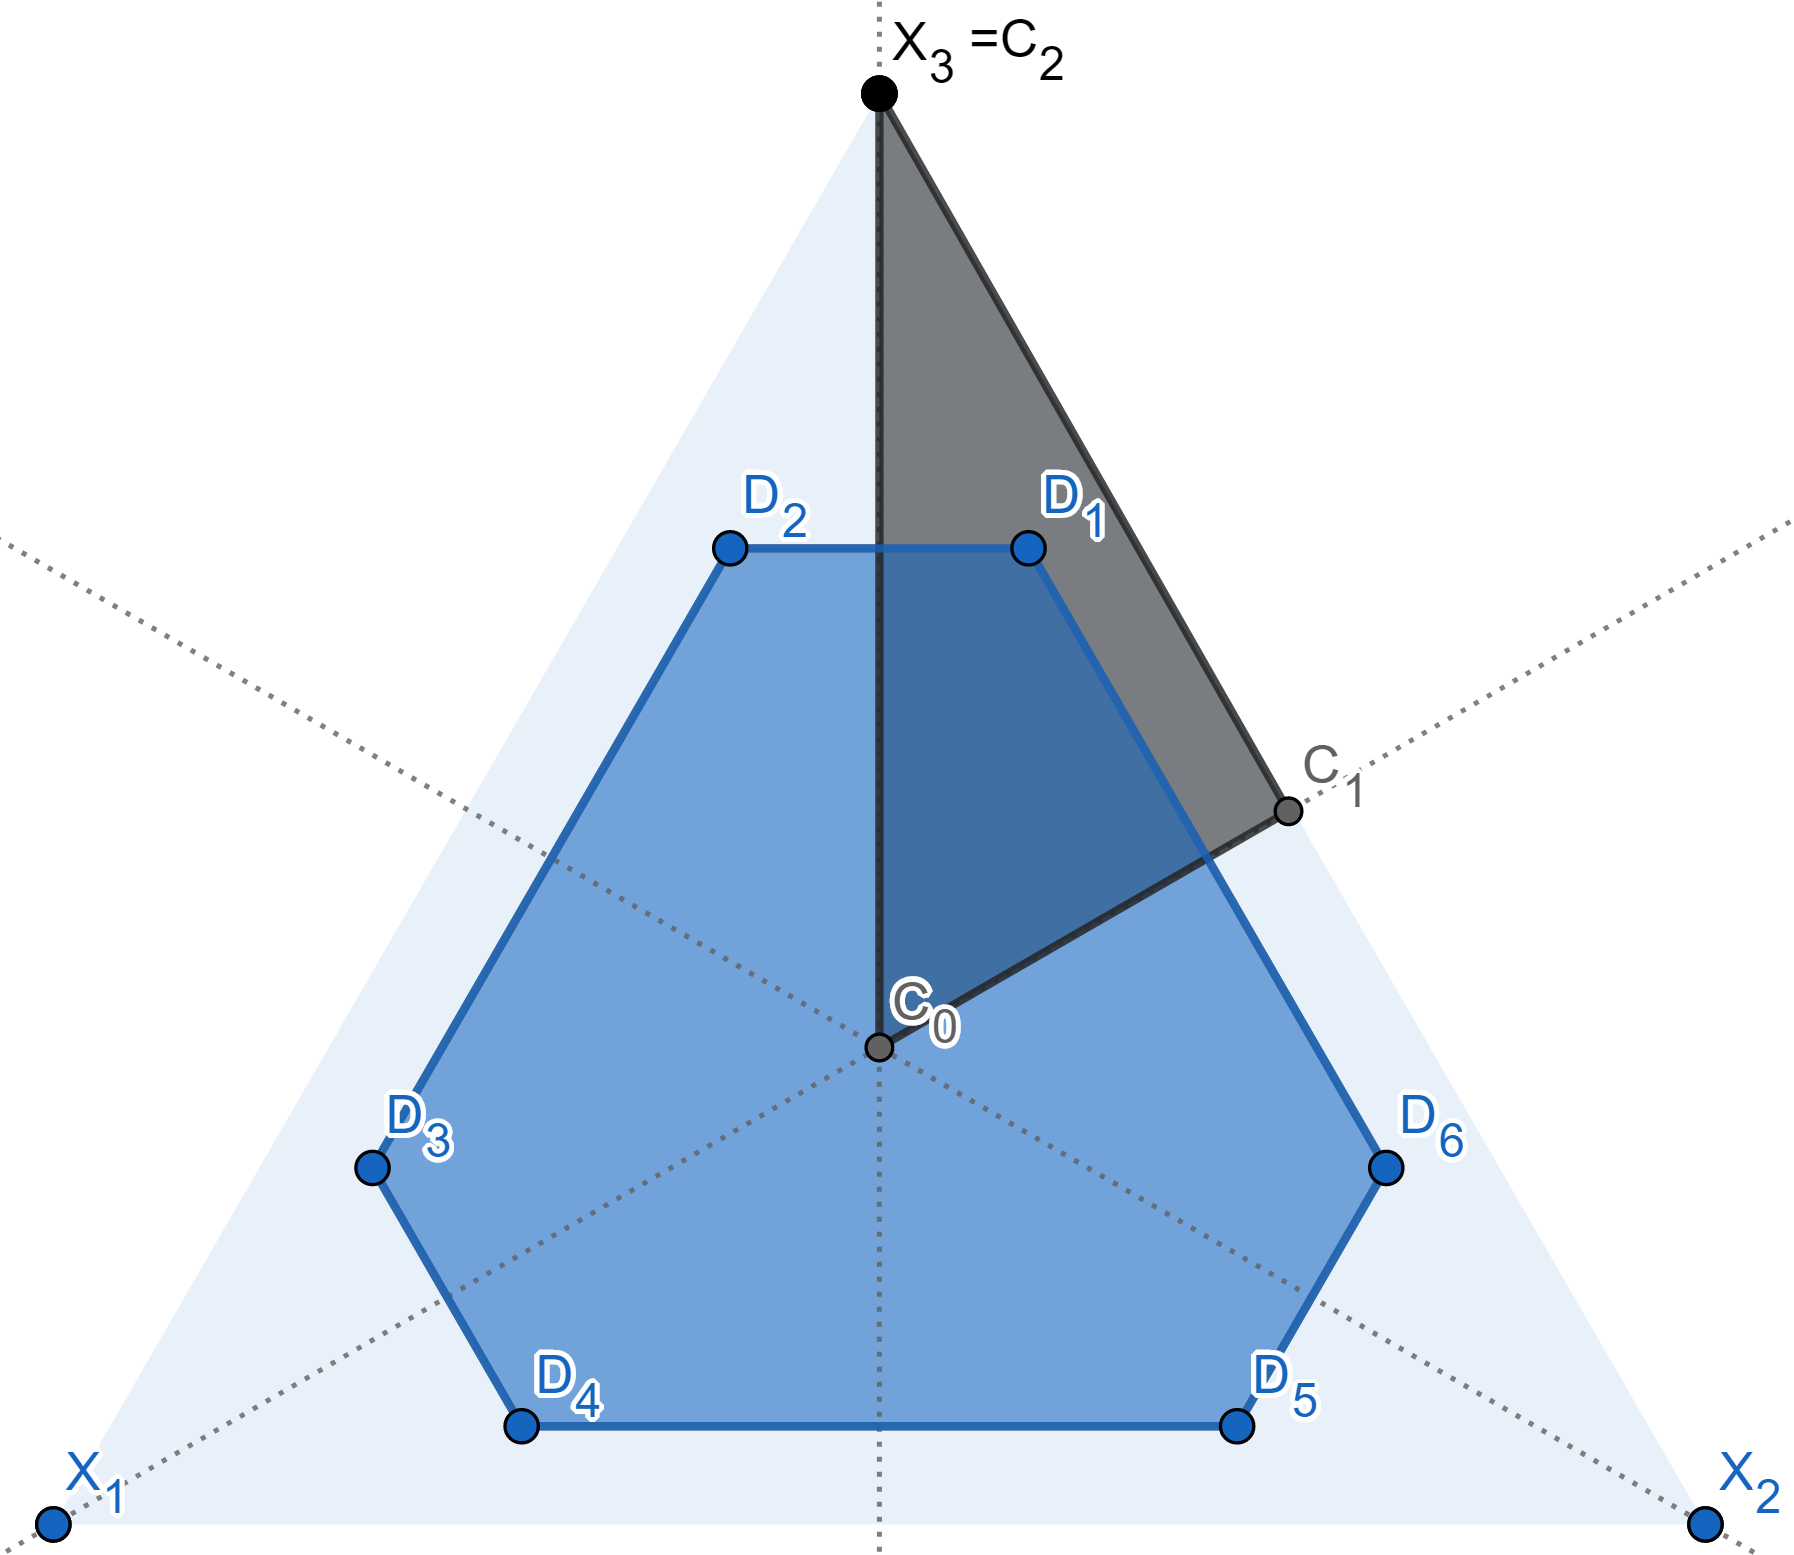
\includegraphics[width=0.7\textwidth]{fundamental_domain}
	\caption{The triangle \(\mathscr{D}\), when \(n=3\). Its three reflection symmetry axes are marked by dashed lines. Its three vertices are \(X_1 = (3,0,0), X_2 = (0,3,0), X_3=(0,0,3)\). Its center is \(C_0 = \mathds{1} = (1,1,1)\). Its fundamental domain is the dark triangle \(C_0C_1C_2\). The hexagon \(D_1D_2D_3D_4D_5D_6\) is generated by the point \(D_1\) in the fundamental domain.}
	\label{fig:fundamental_domain}
\end{figure}

\(\mathscr{D}_0\) can be regarded as a set of representatives from \(\mathscr{D}/\mathbb{G}\), and so, for any \(X\in \mathscr{D}\), there exists a unique element from its orbit that is in \(\mathscr{D}_0\). For any \(\mathscr{F}\subseteq \mathscr{D}\), if \(\mathscr{F}\) is invariant under the actions of \(\mathbb{G}\), that is, $\mathcal{F}$ is law invariant, then it is determined by \(\mathscr{F}\cap \mathscr{D}_0\), since it can be reconstructed by 
\[\mathscr{F} = \bigcup_{\pi \in \mathbb{G}} \left( \mathscr{F}\cap \mathscr{D}_0 \right) \circ \pi.\]

Let \(\Theta = \mathscr{F}\cap\mathscr{D}_0\). For each $p\in \Theta$, let $\mathscr{P}_p$ be the convex hull of $\mathbb{G}(p)$, which is shown in Figure \ref{fig:fundamental_domain} as a hexagon. Then it is geometrically clear that 
\begin{equation}
\mathscr{F} = \bigcup_{p\in \Theta} \mathscr{P}_p = \cl\co\bigcup_{p\in \Theta} \mathscr{P}_p.
\end{equation}
So by \cite[Table 3.3.1]{hiriart-urrutyFundamentalsConvexAnalysis2001}, since $\mathcal{F}$ is the support function of $\cup_{p\in\Theta}\mathscr{P}_p$, which is itself convex and closed, we have
\begin{equation}
\mathcal{F} = \sup_{p\in\Theta} \sigma_{\mathscr{P}_p}.
\end{equation}

Finally, since each $p\in\Theta$ is in $\mathscr{D}_0$, it is a convex sum of the vertices 
$$\left\{
C_0, C_1, ..., C_{n-1}
\right\} = \{q_0, q_1, ... q_{n-1} \}.$$
Thus, there exists a tuple $\theta_p = (\theta_{p, 0}, ..., \theta_{p, n-1})$, such that each $\theta_{p, i} \ge 0$, $\sum_{i = 0}^{n-1}\theta_{p, i} = 1$, and
$$
p = \sum_{i = 0}^{n-1}\theta_{p, i} C_i,
$$
which implies 
$$
\mathscr{P}_p = \co(\mathbb{G}(p)) = \sum_{i = 0}^{n-1}\theta_{p, i}\co(\mathbb{G}(q_i)),
$$
where the second equality is illustrated in Figure \ref{fig:triangle_symmetry}.

\begin{figure}[h]
	\centering
	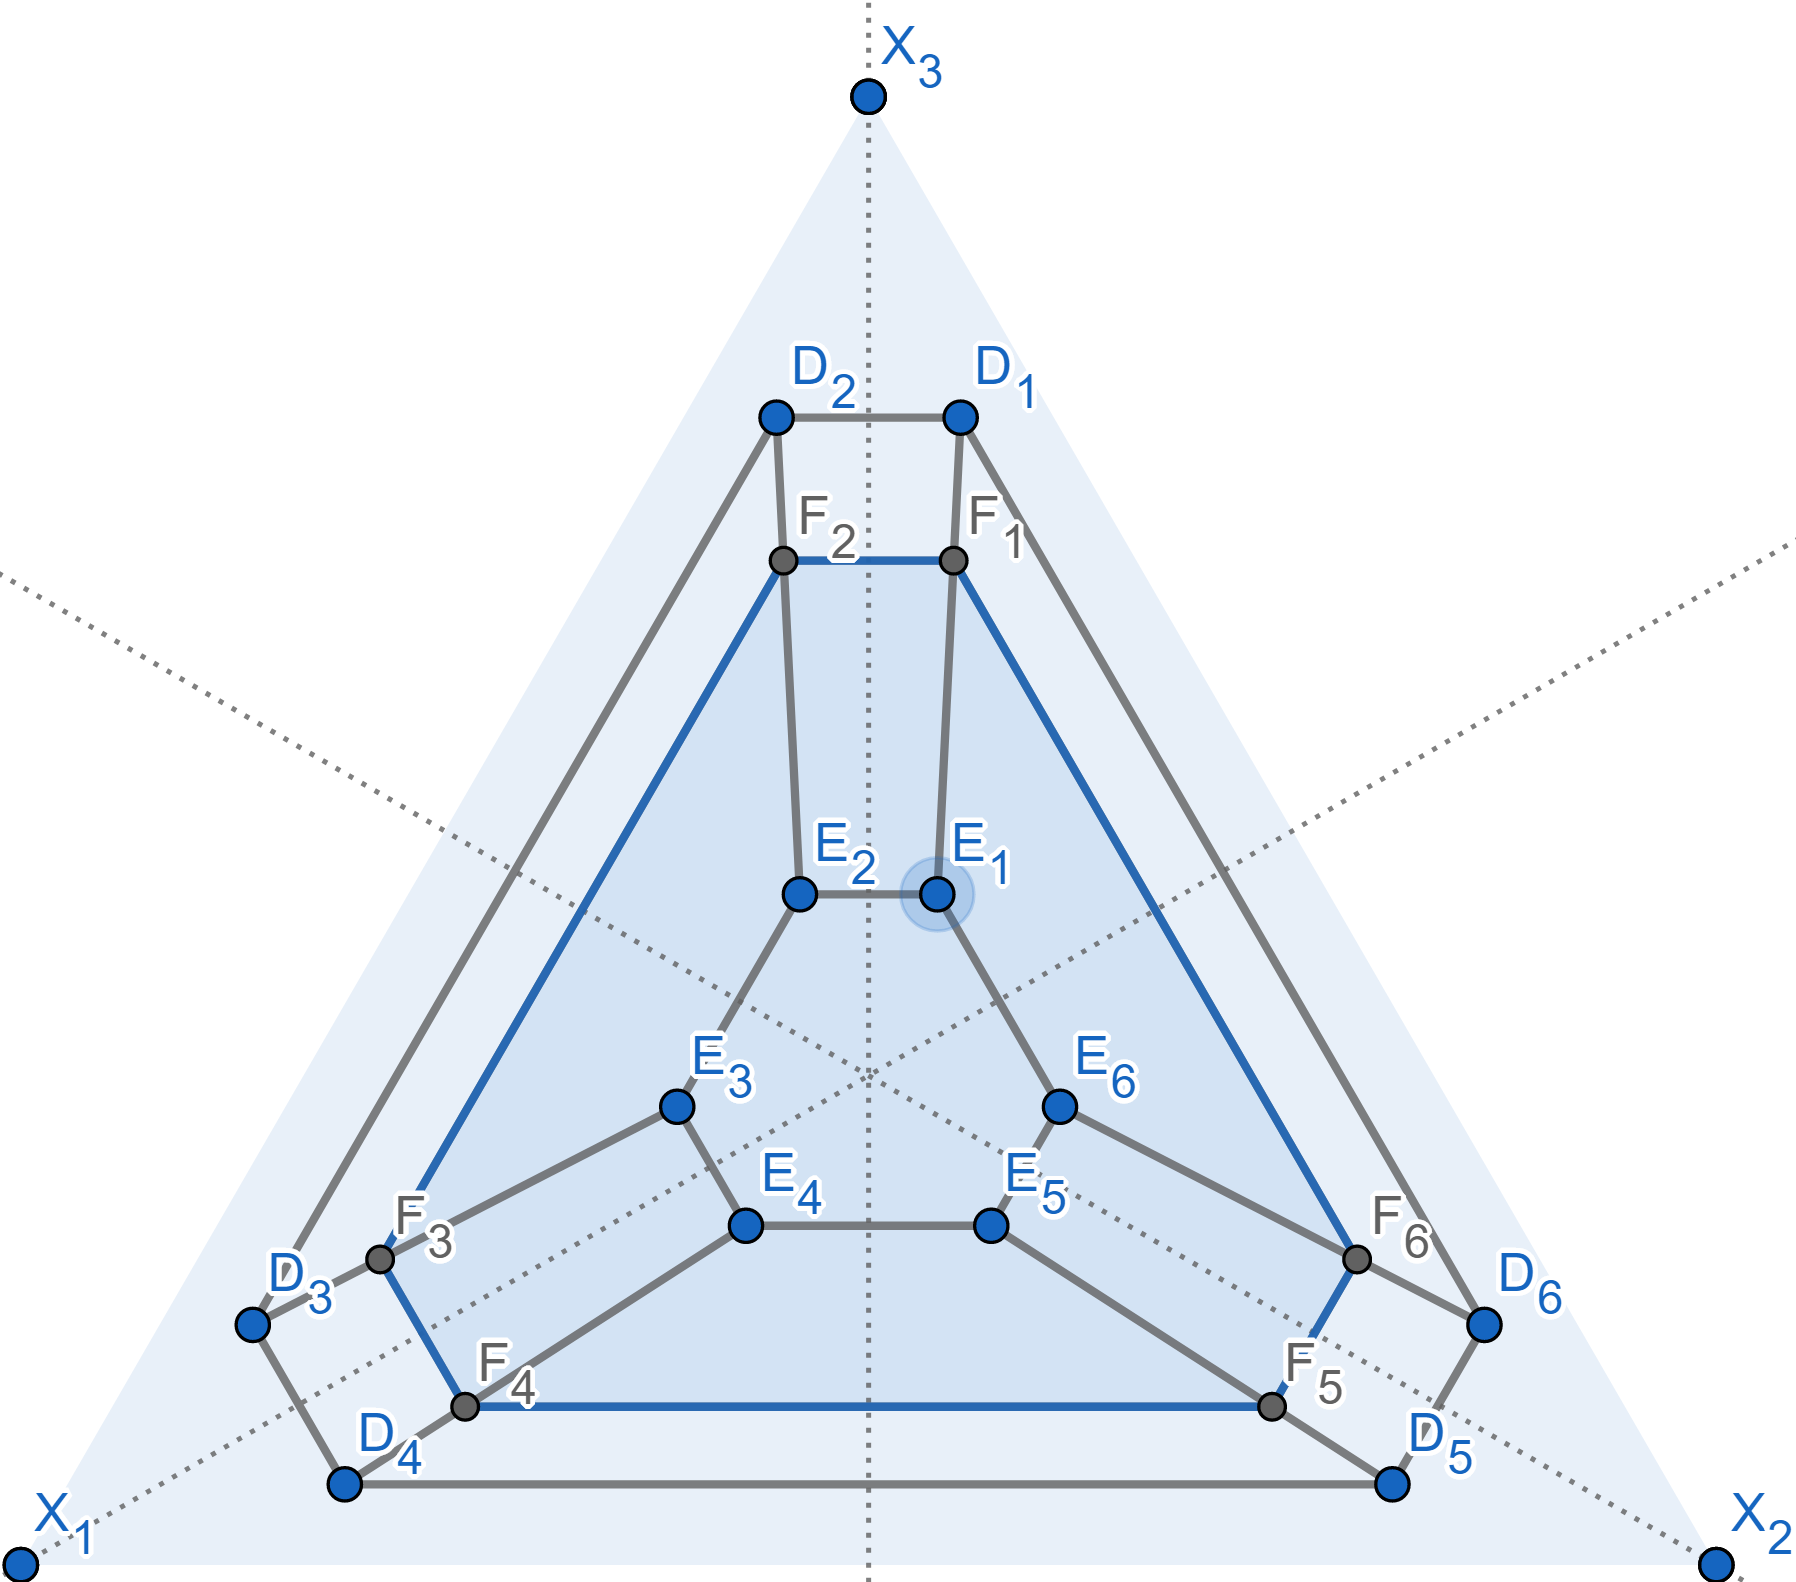
\includegraphics[width=0.6\textwidth]{triangle_symmetry}
	\caption{The triangle \(\mathscr{D}\), with three hexagons generated by the points \(D_1, E_1, F_1\) in the fundamental domain. \(F_1 = \theta D_1 + (1-\theta)E_1\). We have that \(\theta \mathbb{G}(D_1) + (1-\theta) \mathbb{G}(E_1) = \mathbb{G}(\theta D_1 + (1-\theta)E_1)\). In other words, the following two operations commute: interpolating between points in the fundamental domain, and generating a hexagon from a point in the fundamental domain.}
	\label{fig:triangle_symmetry}
\end{figure}

\begin{figure}[h]
	\centering
	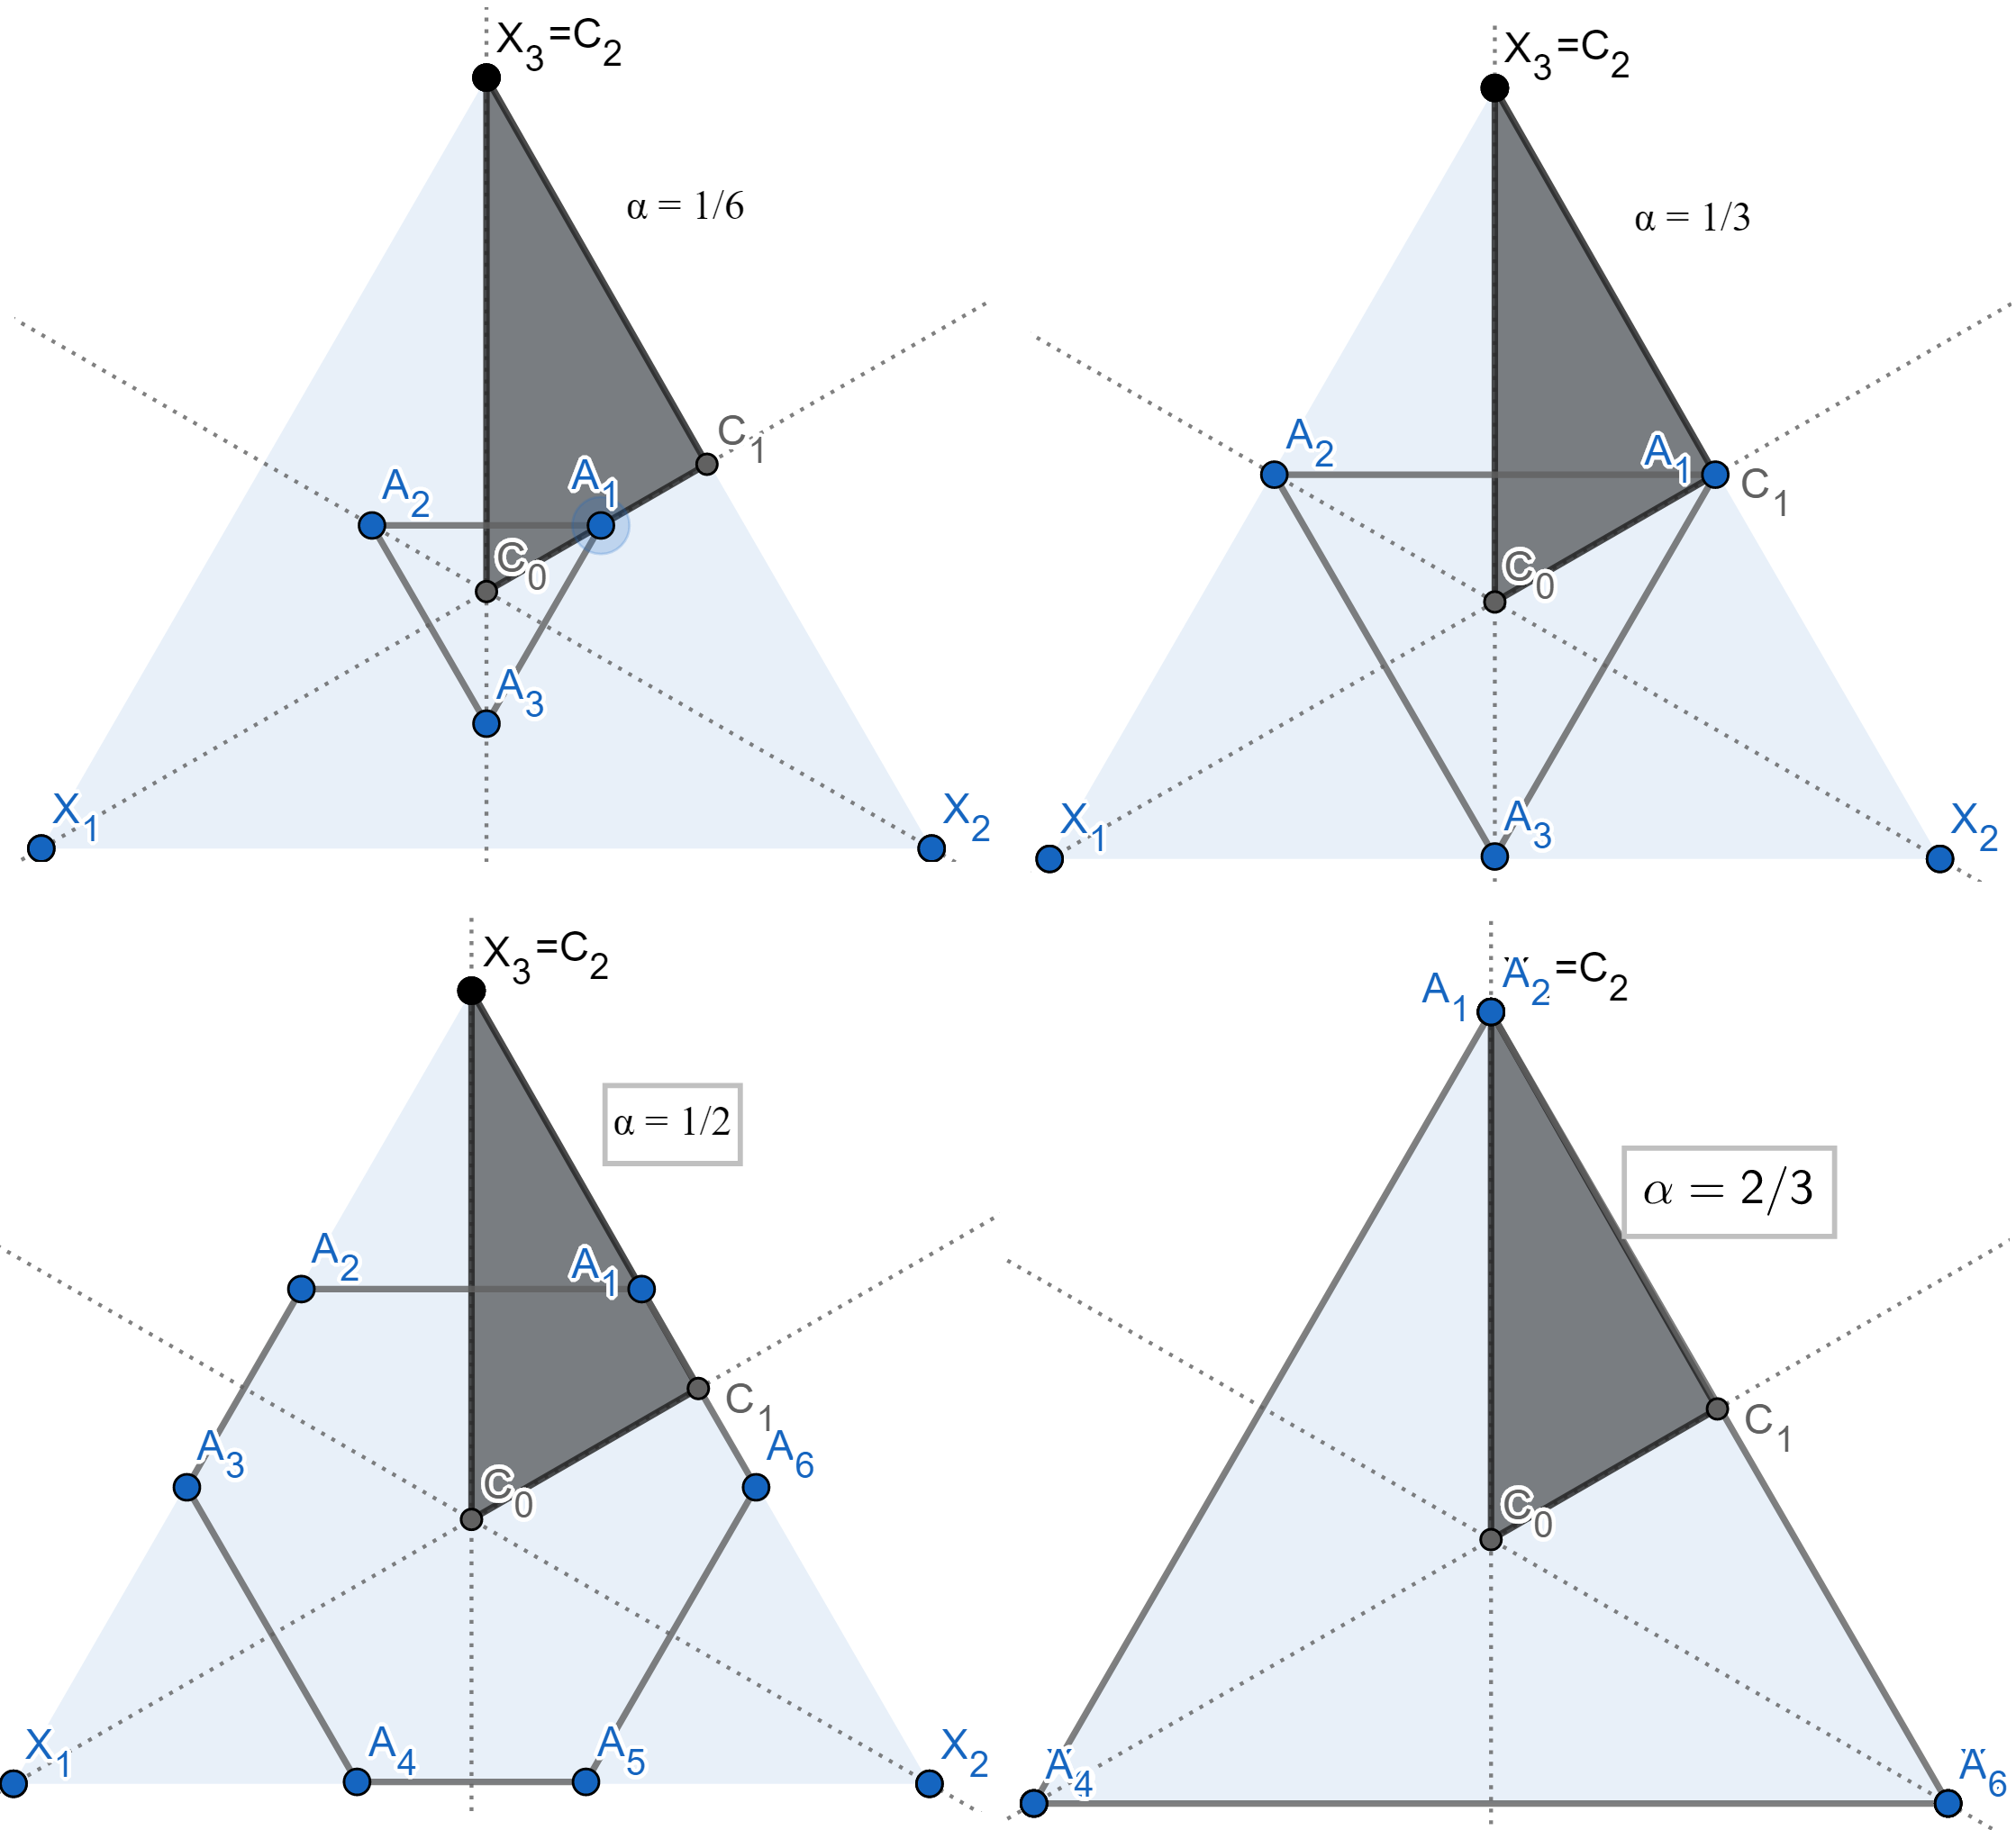
\includegraphics[width=0.7\textwidth]{growing_triangle_merged}
	\caption{\(\mathscr{C}_\alpha\) is generated by \(A_1\), which moves in the fundamental domain as \(\alpha\) increases. When \(\alpha\in [\frac{k}{n}, \frac{k+1}{n}]\), \(A_1\) is on the segment \(C_kC_{k+1}\).}
	\label{fig:growing_triangle_merged}
\end{figure}

Then, since $\co(\mathbb{G}(q_i)) = \mathscr{C}_{\frac i n}$, as illustrated in Figure \ref{fig:growing_triangle_merged}, we have
$$
\mathscr{F} = \bigcup_{p\in\Theta}\mathscr{P}_p = \bigcup_{p\in\Theta} \left(\sum_{i = 0}^{n-1}\theta_{p, i} \mathscr{C}_{\frac in} \right).
$$
Taking the support function on both sides, by \cite[Table 3.3.1]{hiriart-urrutyFundamentalsConvexAnalysis2001} again, 
$$
\mathcal{F} = \sup_{p\in\Theta} \sum_{i = 0}^{n-1}\theta_{p, i} \cvar_{\frac in}.
$$

We summarize the result in a proposition:

\begin{prop}
	If $S = [n]$, $ n \ge 2$, and $\nu$ is uniform on $S$, then any closed, sublinear, translation invariant, law invariant risk measure $\mathcal{F}$ is coherent. 
	
	Let its risk envelope be $\mathscr{F}$. Let $\mathscr{D}_0$ be a fundamental domain of $\mathscr{D}$, defined as in Equation \ref{eq:fundamental_domain}.
	 
	Define $\Theta = \mathscr{D}_0 \cap \partial \mathscr{F}$, then for each $p \in \Theta$, let $\mathscr{P}_p$ be the convex hull of $\mathbb{G}(p)$, then there exists a tuple $\theta_p = (\theta_{p, 0}, ..., \theta_{p, n-1})$, such that each $\theta_{p, i} \ge 0$, $\sum_{i = 0}^{n-1}\theta_{p, i} = 1$, and
	\begin{equation}
	\mathscr{P}_p = \sum_{i = 0}^{n-1}\theta_{p, i} \mathscr{C}_{\frac in},
	\end{equation}
	and we have the Kusuoka representation 
	\begin{equation}
	\mathcal{F} = \sup_{p\in\Theta} \sum_{i = 0}^{n-1}\theta_{p, i} \cvar_{\frac in}.
	\end{equation}
\end{prop}

\subsection{The case of nonuniform probability on \(S\)}
\label{sec:nonuniform_space}
Let \(S = [n]= \{1, 2, \cdots , n\} \), where \(n \) is an integer at least \(2\). Let \(\nu\) be a nonuniform probability measure on \(S\). 

For this section, we do a specific example, which is a sufficiently illustrative example for the general \(n \ge 2\) cases.

Let \(n=4\); let \(\nu \) be defined by
\[\nu: 1\mapsto \frac{1}{6}, 2\mapsto \frac{1}{6}, 3\mapsto \frac{1}{3}, 4\mapsto \frac{1}{3}\]
Thus, its symmetry group \(\mathbb{G}\) has \(4\) elements, and breaks \(S\) into two orbits: \(\{1, 2\} \) and \(\{3,4\} \). 

Let the centroids of the orbits be \(A = \frac{X_1 + X_2}{2}, B = \frac{X_3 + X_4}{2}\), and let \(C = \mathds{1}\).

Take any closed convex \(\mathscr{F} \subseteq \mathscr{D}\) that contains \(C\) in its interior (relative to \(\mathscr{D}\)). Connect \(A, B\), making a line passing \(C\) and intersecting \(\partial\mathscr{F}\) at two points $D, E$. This is shown in Figure \ref{fig:tetrahedron_homothety}.

Define the \textbf{line ratio} of \(\mathscr{F}\) be 
$$LR(\mathscr{F}) = \overline{DC} : \overline{CE},$$
and let $r_0 = LR(\mathscr{D}) = \overline{AC} : \overline{CB}$. Without loss of generality, assume that $\overline{AC} \ge \overline{CB}$, so that $r_0 \ge 1$. 

In our particular example, it happens that $\overline{AC} = \sqrt{10}, \overline{CB} = \sqrt{10}/2$, so $r_0 = 2$.

For small $\alpha > 0$, $\mathscr{C}_\alpha$ is an inverted homothetic image of $\mathscr{D}$, so $LR(\mathscr{C}_\alpha) = 1/r_0$. For big $\alpha < 1$, we have $D = A$ and $E = B$, so $LR(\mathscr{C}_\alpha) = r_0$. Between them, we have 
$$\forall \alpha\in (0, 1], LR(\mathscr{C}_\alpha)\in [1/r_0, r_0].$$
This is in fact true in general for all Kusuoka-representable sets:

\begin{prop}[Kusuoka set line ratio]
Take any nontrivial Kusuoka set, as defined in Equation \ref{eq:kusuoka_set}:
$$
\mathscr{F} = \cl\co\bigcup_{\theta \in \Theta}\int_0^1 \mathscr{C}_\alpha dm_\theta(\alpha),
$$
and assume it is nontrivial, that is, $\mathscr{F}\neq \{\mathds{1}\}$. Then $LR(\mathscr{F}) \in [1/r_0, r_0]$.
\end{prop}
\begin{proof}\textit{(Sketch)} Refer to Figure \ref{fig:tetrahedron_homothety}.

	Translate the origin of the coordinate frame to point $C$. So, for example, $A$ in the new coordinate frame is $(2,2,-1,-1)$.
	
	For each point $P\in\mathbb{R}^n$, let $f(P)$ be its projection onto the line $AB$, and define $d(P)$ to be the directed distance from $C$ to $f(P)$. So, for example, $d(A) = \sqrt{10}, d(B) = -\sqrt{10}/2$.
	
	Since the affine subspaces spanned by $\{X_1, X_2\}$ and spanned by $\{X_3, X_4\}$ are perpendicular to line $AB$, the projection of $\mathscr{D}$ onto the line $AB$ is the line segment $[A,B]$.
	
	Then, for any $\alpha \in (0, 1]$, 
	$$f(\mathscr{C}_\alpha) = [D_\alpha, E_\alpha] = AB \cap \mathscr{C}_\alpha,$$
	where we append the subscript $\alpha$ to $D, E$ to denote its association with $\mathscr{C}_\alpha$. Then the line ratio of $\mathscr{C}_\alpha$ is 
	$$LR(\mathscr{C}_\alpha) = -\frac{d(D_\alpha)}{d(E_\alpha)}\in[1/r_0, r_0]$$
	
	For any probability measure $m_\theta$ on $[0, 1]$, let $\mathscr{P}_\theta = \int_0^1 \mathscr{C}_\alpha dm_\theta(\alpha)$. Then $f(\mathscr{P}_\theta) = [D_\theta, E_\theta]$, where 
	$$d(D_\theta) = \int_0^1 d(D_\alpha) dm_\theta(\alpha), \quad d(E_\theta) = \int_0^1 d(E_\alpha) dm_\theta(\alpha).$$
	Thus, 
	$$LR(\mathscr{P}_\theta) = -\frac{d(D_\theta)}{d(E_\theta)}\in[1/r_0, r_0].$$
	
	Finally, let $\mathscr{F} = \cl\co\bigcup_{\theta \in \Theta}\mathscr{P}_\theta$, we have
	$$d(\mathscr{F}) = \left[\inf_{\theta \in \Theta} d(E_\theta), \sup_{\theta \in \Theta} d(D_\theta)\right],$$
	and so
	$$LR(\mathscr{F}) \in [1/r_0, r_0].$$
\end{proof}


\begin{figure}[h]
	\centering
	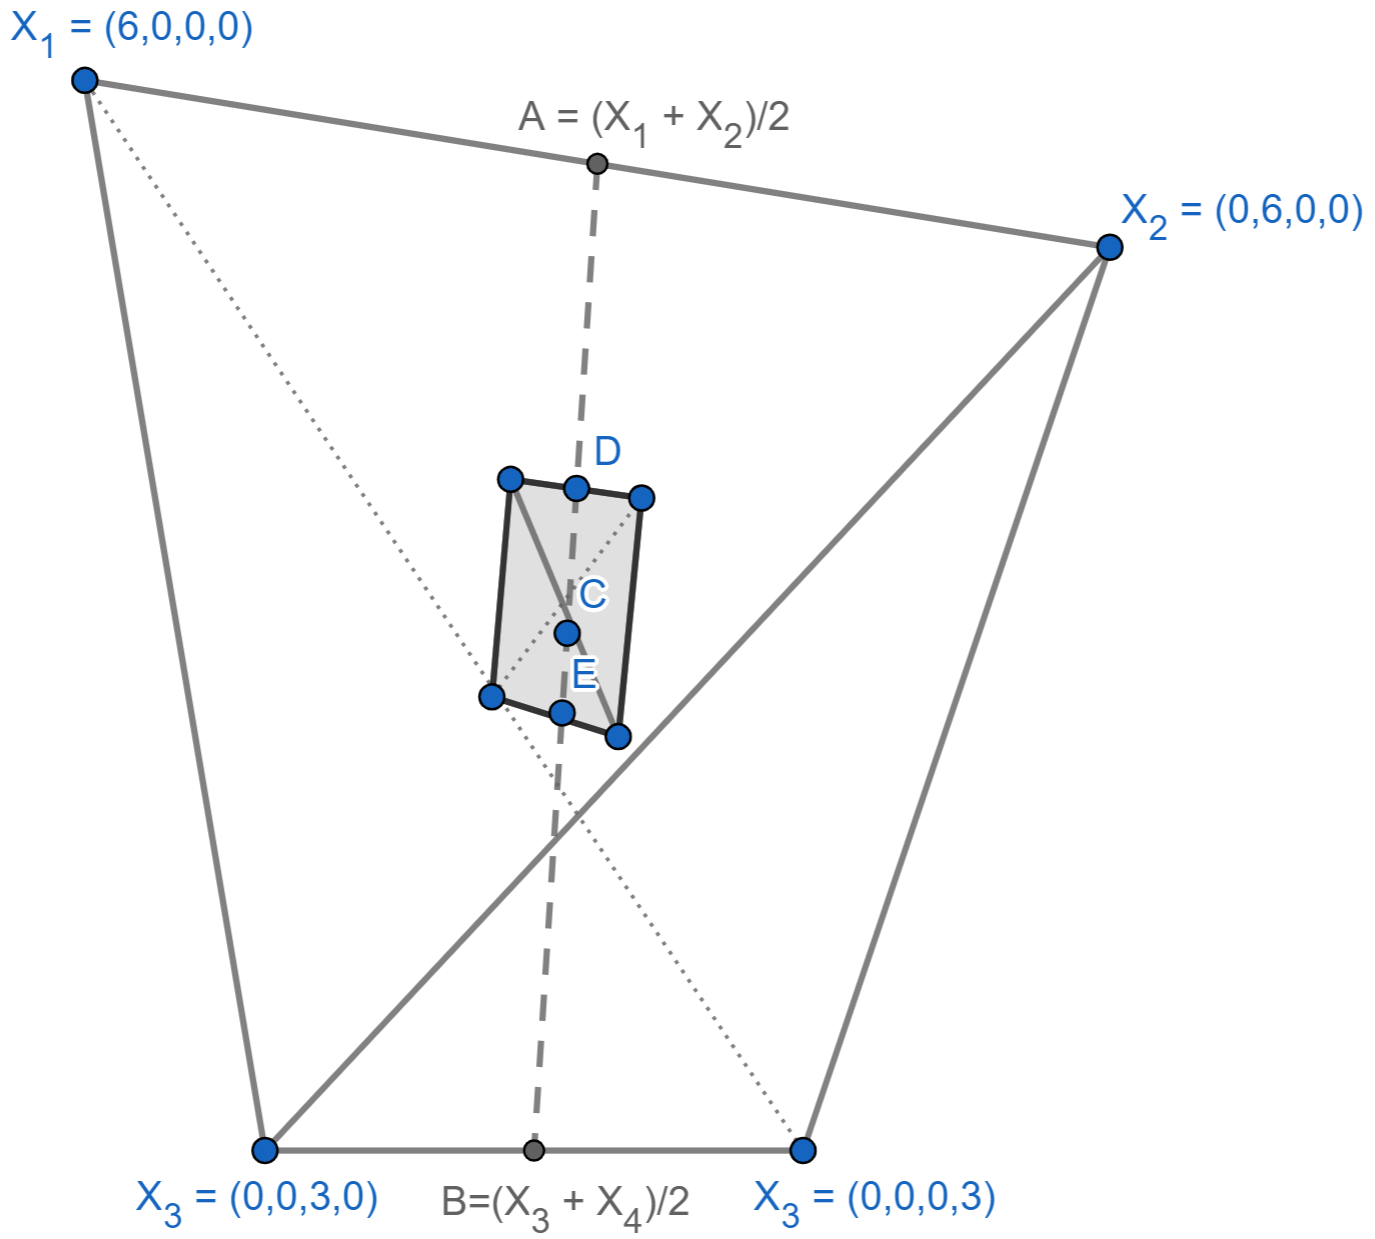
\includegraphics[width=0.7\textwidth]{tetrahedron_homothety}
	\caption{When \(n = 4\), \(\mathscr{D}\) is a tetrahedron, centered at \(C = \mathds{1} = (1,1,1,1)\). With the \(\nu\) defined in the text, the tetrahedron is not regular. For a small \(\alpha\), \(\mathscr{C}_\alpha\) is a small homothetic copy of \(\mathscr{D}\), here drawn in the center in gray. The "line ratio" is obtained by connecting \((X_1 + X_2)/2\) and \((X_3 + X_4)/2\), cutting \(\mathscr{C}_\alpha\) at \(D, E\), then defining the ratio as \(\overline{DC} : \overline{CE}\).}
	\label{fig:tetrahedron_homothety}
\end{figure}

\begin{figure}[h]
	\centering
	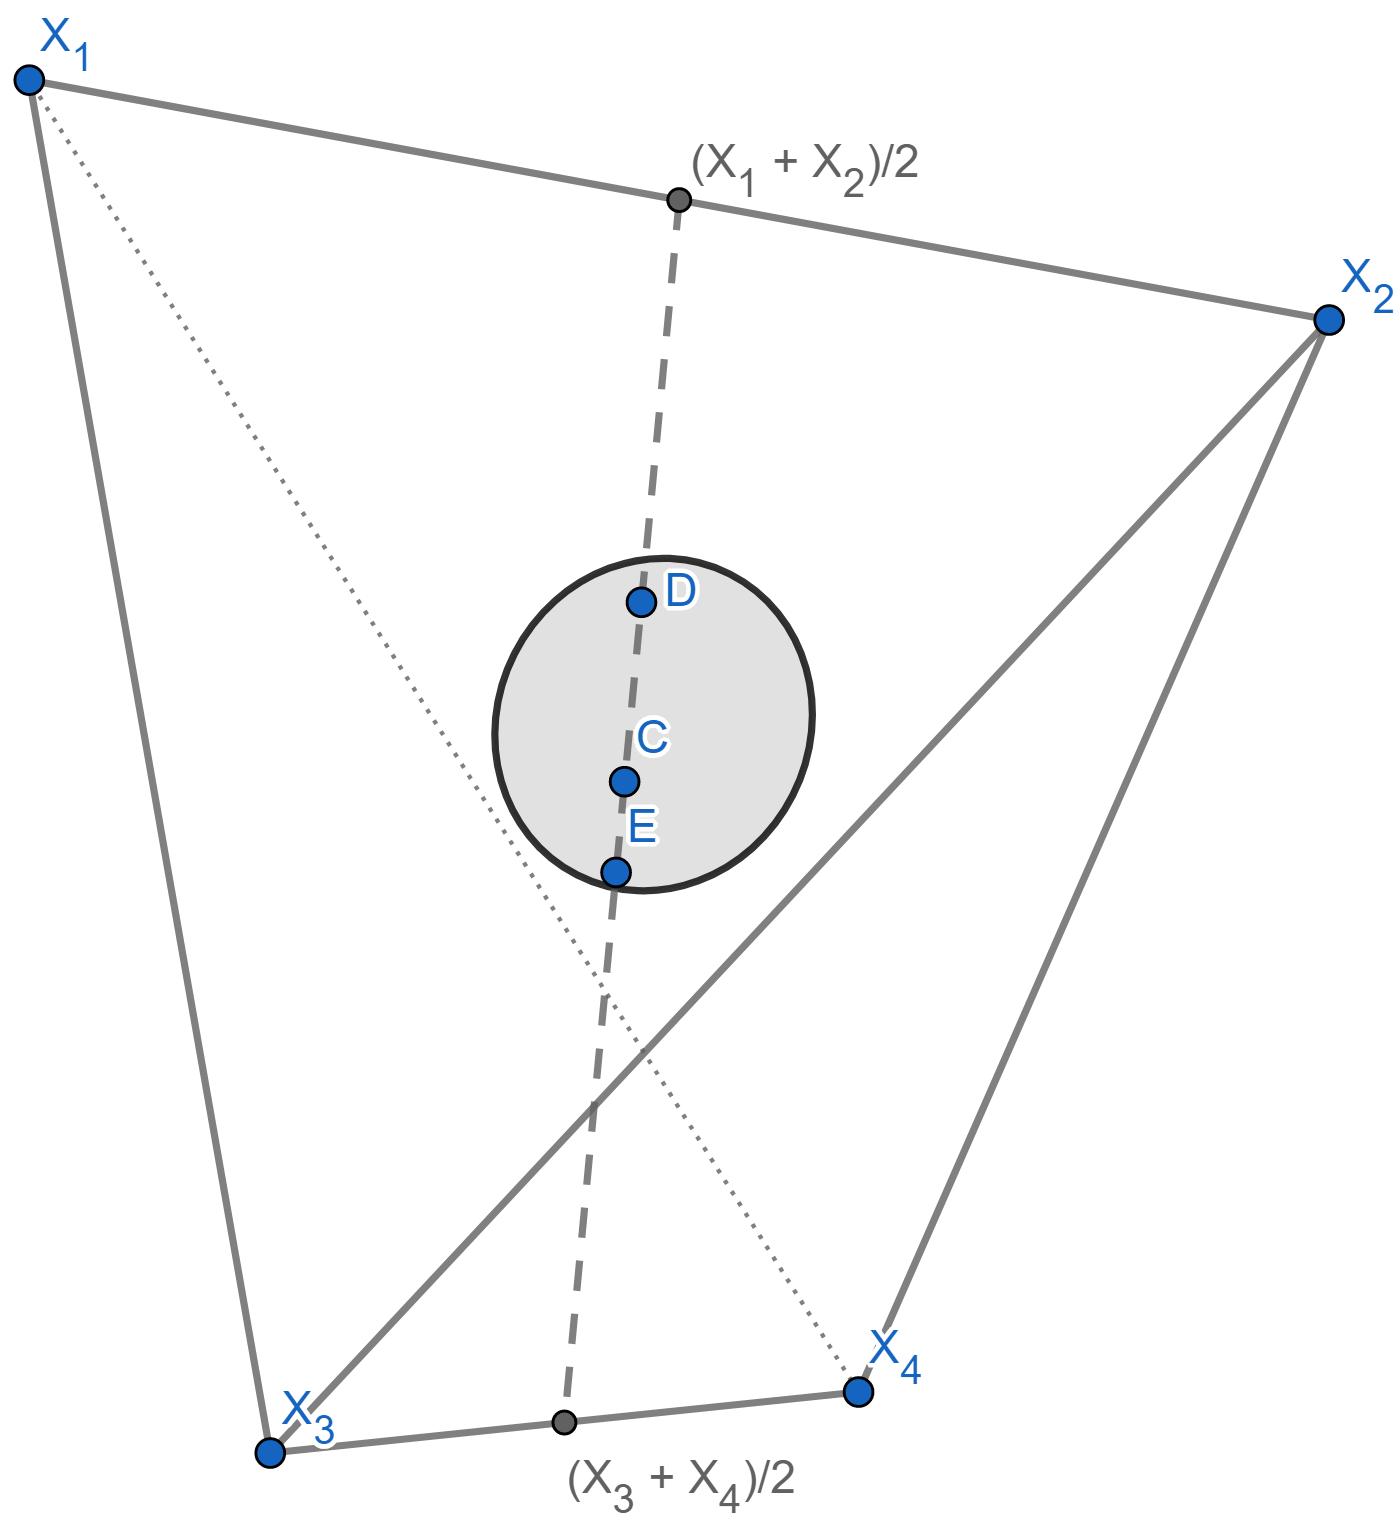
\includegraphics[width=0.5\textwidth]{tetrahedron_irregular}
	\caption{To construct a closed, law invariant, strictly risk averse, coherent risk measure that has no Kusuoka representation, take a small closed ball around \(\mathds{1}\), then shift it along the line connecting \((X_1 + X_2)/2\), \((X_3 + X_4)/2\), until its line ratio moves out of the bound.}
	\label{fig:tetrahedron_irregular}
\end{figure}

To violate this line ratio, simply take a closed ball of very small radius \(r\), in \(\mathscr{D}\) around \(\mathds{1}\), then shift it by \((1-\epsilon)r\) in the direction of \(\frac{X_1 + X_2}{2} - \frac{X_3 + X_4}{2}\). Let the resulting set be \(\mathscr{F}\), then \(\mathcal{F} = \sigma_{\mathscr{F}}\) is a closed, law invariant, strictly risk averse, coherent risk measure that can be arbitrarily close to \(\mathbb{E}\), and yet has no Kusuoka representation.

Also, note that if we shift the ball by \((1 + \epsilon)r\) instead, then we obtain a closed, law invariant, coherent risk measure that is not risk averse, and can be arbitrarily close to \(\mathbb{E}\). This contrasts with the case of uniform probability on \(S\), where any law invariant, coherent risk measure is either \(\mathbb{E}\) or strictly risk-averse.

We record this formally as:

\begin{prop}
	If $S = [n]$, $ n \ge 2$, and $\nu$ is nonuniform on $S$, then there exists closed, law invariant, risk averse, coherent risk measures that are arbitrarily close to $\mathbb{E}$, and yet have no Kusuoka representations.
\end{prop}

